\documentclass[conference]{IEEEtran}
\IEEEoverridecommandlockouts
% The preceding line is only needed to identify funding in the first footnote. If that is unneeded, please comment it out.
\usepackage{cite}

\usepackage{amsmath,amssymb,amsfonts}
\usepackage{algorithmic}
\usepackage{graphicx}
\usepackage{textcomp}
\usepackage{xcolor}

\DeclareGraphicsExtensions{.pdf,.jpeg,.png,.eps}
\graphicspath{{./figures/}}

\usepackage{multirow}

\usepackage{colortbl}

    
\begin{document}

\title{IEEE 802.15.4 Historical Evolution and Trends}
\author{
\IEEEauthorblockN{Alberto Gallegos Ramonet\textsuperscript{*}, Taku Noguchi** }
\IEEEauthorblockA{\textit{College of Information Science and Engineering} \\
\textit{Ritsumeikan University}\\
Shiga, Japan \\ \textbf{ramonet@fc.ritsumei.ac.jp}, \textbf{noguchi@is.ritsumei.ac.jp} }
}

\maketitle

\begin{abstract}
For several years, the IEEE 802.15.4 standard has been the backbone of applications with low latency and small energy consumption requirements. Its popularity has made it the de facto standard for this type of network communication, and the IEEE 802.15.4 standard will continue to play an important role in the Internet of Things (IoT) revolution. The standard has existed for the past 15 years and its applications have evolved over the years. In this paper, we present a concise and chronological description of the standard highlighting each feature that has been introduced over the years. A compendium of this kind can be valuable to researchers working on implementations and improvements and to users seeking a general reference. This is relevant now more than ever because the standard must coexist with hundreds of other standards that are also constantly evolving. As presented in this document and despite its popularity and importance, there are very few capable IEEE 802.15.4 simulators and these are often outdated and incomplete. The aim of this paper is to provide a quick reference but also present the evolution of the standard and its future directions. Similarly, we hope that this study fosters the creation of new implementations, particularly new simulations modules.
 
\end{abstract}

\begin{IEEEkeywords}
LR-WPAN, protocols, survey, WSN, simulations, Zigbee, IEEE 802.15.4
\end{IEEEkeywords}

\section{Introduction}
Networks in our homes, offices, and mobile devices are constantly evolving. Not all network-enabled devices are connected to the Internet nor do they need to be. For example, devices found in our homes such as electric doors, televisions, and air conditioning systems may benefit from sharing information between each other, but in most cases, using the internet to connect these appliances may not be a cost effective solution because of the unnecessary added complexity, communication overhead, and unwanted privacy concerns. In such cases, internet independent networks are a preferred choice. Independent networks used in Wireless Sensor Networks (WSN) are an example. The IEEE 802.15.4 standard was released in 2003 \cite{std2003} to describe such types of networks. WSN have been developed for strict power constraints in specialized applications with low latency or for applications characterized by disruptive connections. In this paper, we present a chronological description of the IEEE 802.15.4 standard known as Low-Rate Wireless Personal Area Networks (LR-WPAN). Furthermore, this study describes the MAC behaviors and the available options of its physical layers and also clarifies the often overlooked formation of mesh networks and available simulations. Despite the popularity of the IEEE 802.15.4 standard, to our knowledge, there are no similar compendiums that present a complete evolutionary summary of the standard. This document is relevant for multiple reasons. For instance, the standard includes an extensive collection of physical layer options and MAC layer improvements that are not available in all revisions. In some cases, drastic changes make certain implementations obsolete or incompatible. Moreover, official standard descriptions assume the knowledge of prior revisions, making such documents hard to navigate without having a general idea of the standard such as the one presented in this study. Consequently, new improvements and implementations can be convoluted and time consuming. It is also worth noting that implementations and simulations of the standard are considerably behind the most recent revisions. For example, Zigbee, arguably the most popular commercial implementation of the IEEE 802.15.4 standard, only until recently (V3.0) supported the 2011 revision of the standard \cite{nxpManual} despite the existence of amendments as late as 2018. Owing to these reasons, we believe that users and implementers will find the summary presented in this document relevant and useful. This paper is organized as follows: Section \ref{evolutionStd} describes the complete evolution of the IEEE 802.15.4 standard, highlighting differences between each revision. %A summary of the PHY layers conforming the standard can be located %at Table \ref{tab:phyTable} at the end of this Section. 
Section \ref{implementationStd} presents a brief description of some of the most popular simulation implementations, which is followed by our conclusions.


\section{Evolution of the IEEE 802.15.4 Std.} \label{evolutionStd}

\subsection{IEEE 802.15.4 (2003)}\label{wpan2003}

Initially released in 2003, the IEEE 802.15.4 standard \cite{std2003} defines the interconnection of LR-WPAN devices. It uses the Carrier Sense Multiple Access with Collision Avoidance (CSMA/CA) to access the medium and support star and peer-to-peer topologies. Its architecture layout can be described in terms of blocks based on the open systems interconnection (OSI) seven-layer model in which each block (also called layer) has a specific task and provides services to upper blocks. The PHY layer (Physical layer or layer 1) contains the radio frequency (RF) transceiver with a low-level control mechanism. The 2003 standard defines two PHYs: a 2450 MHz direct sequence spread spectrum (DSSS) with a maximum data rate over-the-air of 250 kb/s and the less commonly used 915 Mhz and 868 Mhz bands with data rates of 40 kb/s and 20 kb/s, respectively. 
The MAC layer (Media Access Control or layer 2) provides access to the physical channel. Although the standard primarily consists of these two layers, the standard also describes an additional Logical Link Control (LLC) and a Service Specific Convergence Sublayer (SSCS) between the MAC layer and the next layer to facilitate communication. The implementation details of the upper layers are beyond the scope of the standard. Transmission of data can be performed with or without the help of beacon messages. In a beacon-enabled Personal Area Network (PAN), a single Full Functional Device (FFD) acts as a PAN coordinator while the remaining devices are either FFD or Reduced Functional Devices (RFD). Different from a beacon-enabled PAN, in a non-beacon enabled PAN, devices compete for the medium at all times. 
% The popularity of the 2450MHz over the other two PHY is attributed to 3 factors: Its %higher data rate of 250 kb/s, the fact that 2450Mhz was a free spectrum  in most of the %world at the time of its release and the fact that the other two bands used a different %modulation technique which from the point of view of physical implementation presented %challenges to the sellers.
\begin{figure}[!htb]
\centering
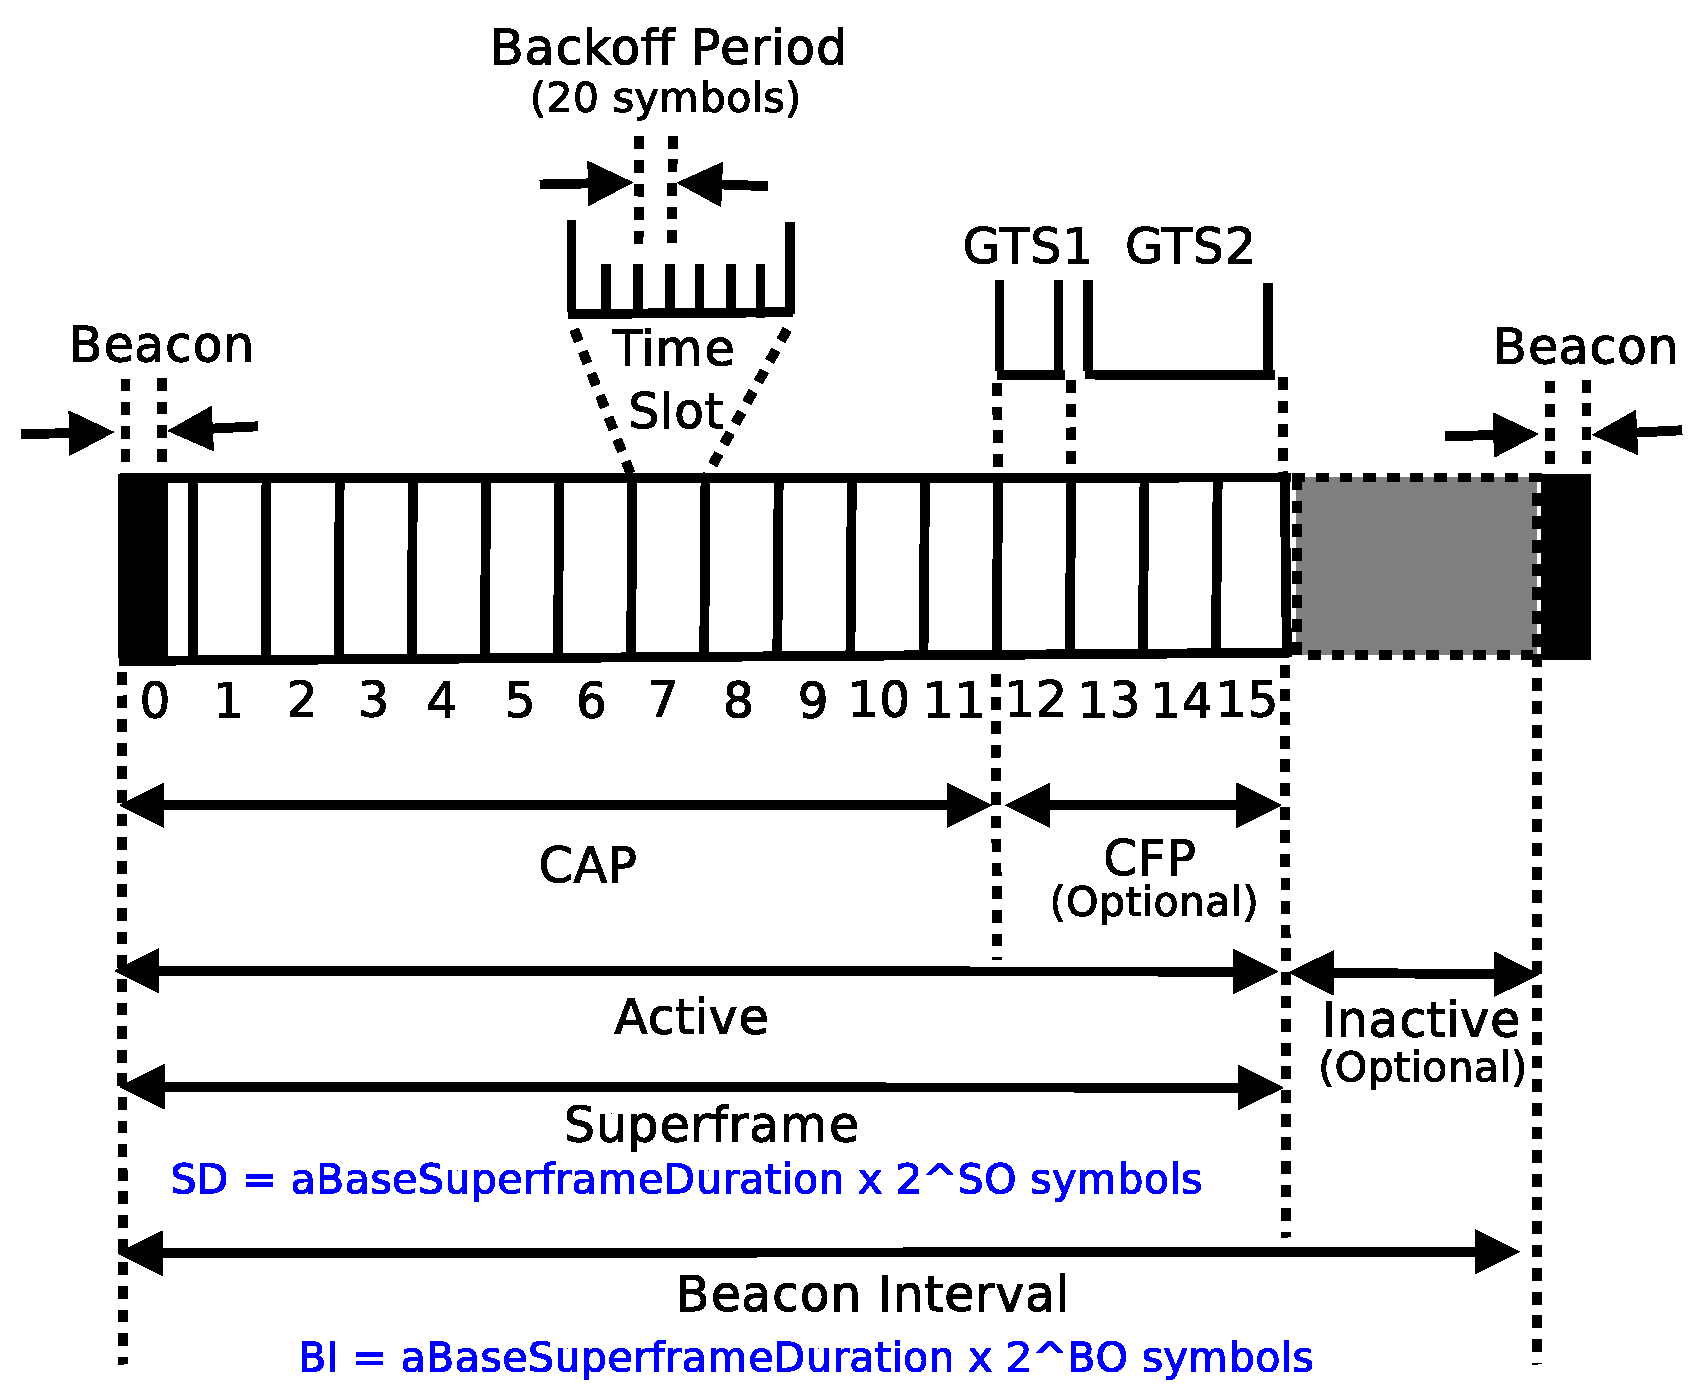
\includegraphics[scale=.28]{superframe}
\caption{Beacon-enabled mode superframe description.}
\label{fig:superframe}
\end{figure}

In a beacon-enabled PAN, the PAN coordinator transmits in intervals beacons containing a \textit{superframe} structure that defines an active period of time between beacons. The superframe is used to realize synchronized communication between the PAN devices. Figure \ref{fig:superframe} summarizes the structure of a superframe. A superframe is formed by 16 time slots in which a beacon is always sent during the first time slot. Similarly, each of these time slots consist of 20 \textit{symbols}. A symbol is a representation of time in bits. For example, in the IEEE 802.15.4 standard that uses a O-QPSK modulation, 1 symbol is equivalent to 4 bits (0.016 ms in a 250-kbps connection). A Beacon Interval (BI) is defined by  \mbox{$aBaseSuperframeDuration \times 2^{BO}$} symbols. The Beacon Order (BO) is a user defined integer between 0 and 14 and $aBaseSuperframeDuration$ is a constant equal to 960 symbols. The BI includes both the active and inactive periods of time. The inactive period is optional with no transmissions, and the radio transceiver can be turned off to preserve energy. The active portion depends on the user defined variable Superframe Order ($SO$) and its length is described by the Superframe Duration (SD). The SD is equal to \mbox{$aBaseSuperframeDuration \times 2^{SO}$} symbols for \mbox{0 $\leq$ $SO$ $\leq$ $BO$ $\leq$ 14}. The active portion is further divided into a Contention Access Period (CAP) and Contention Free Period (CFP). In the CAP, devices contend for the transmission of data using a slotted version of the CSMA/CA algorithm. Time slots are formed by multiple \textit{backoff periods} \mbox{(1 backoff period is equivalent to 20 symbols)}. Operations within the CAP always occur on the boundary of a backoff period. The CFP is an optional part of the active period but if it is used, it must always be located at the end of the active period. The CFP is divided into Guaranteed Time Slots (GTS), which are assigned to specific devices for transmission without contention. A maximum of 7 GTS can be assigned. Their length directly depends on the maximum size of the CFP and the total number of GTS assigned.
\begin{figure}[!htb]
\centering
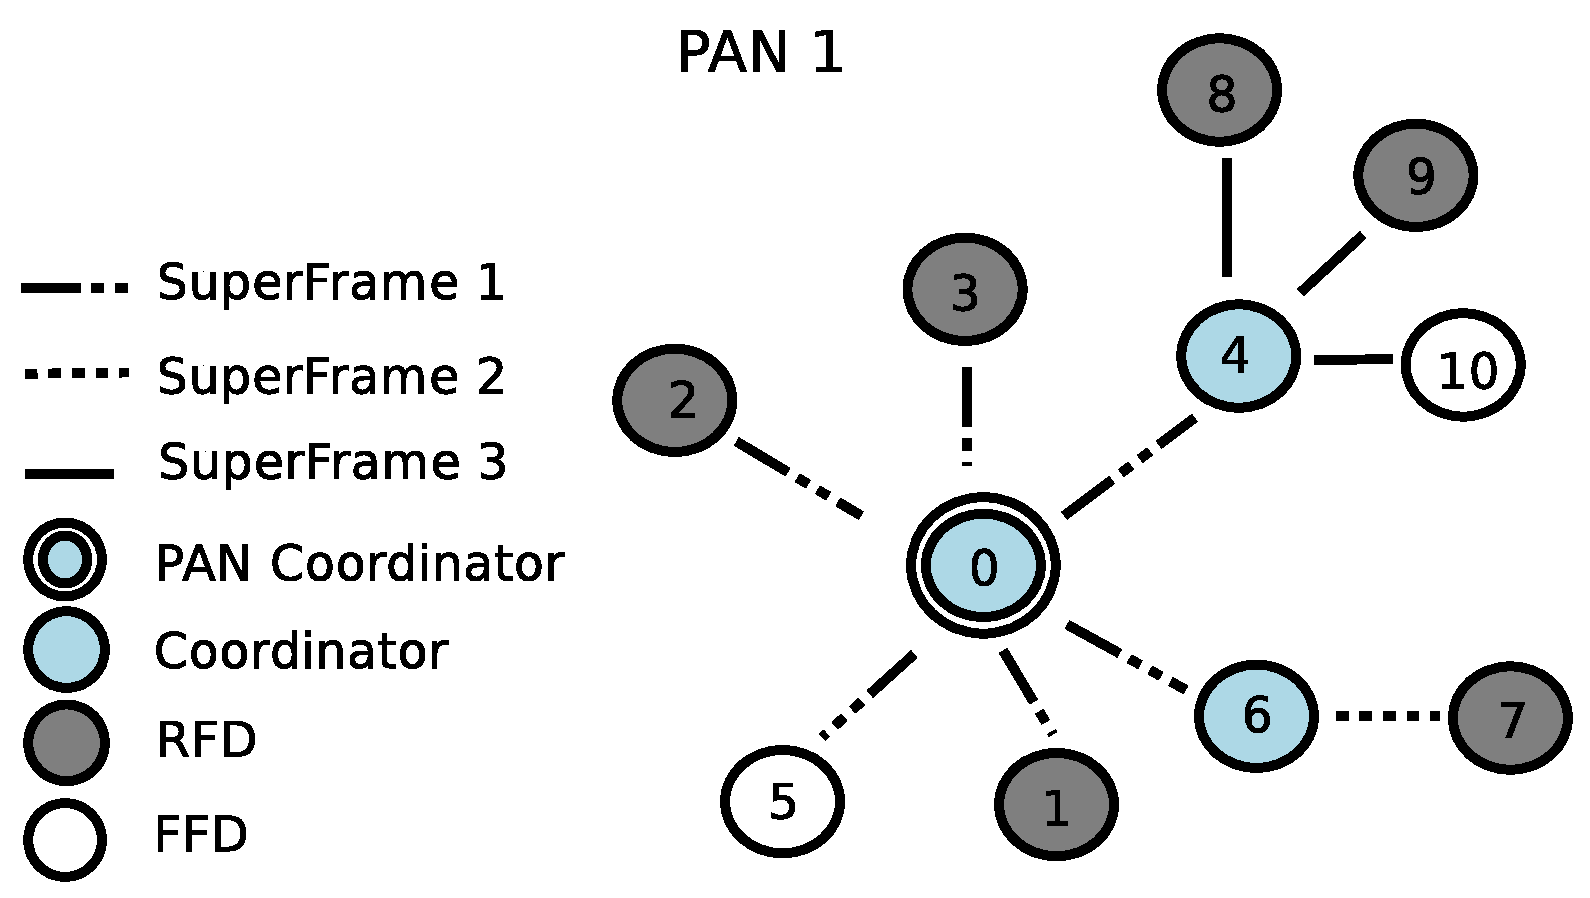
\includegraphics[scale=.28]{peerTopology}
\caption{ IEEE 802.15.4 Mesh topology in single PAN.}
\label{fig:peerTopology}
\end{figure}

\begin{figure}[!htb]
\centering
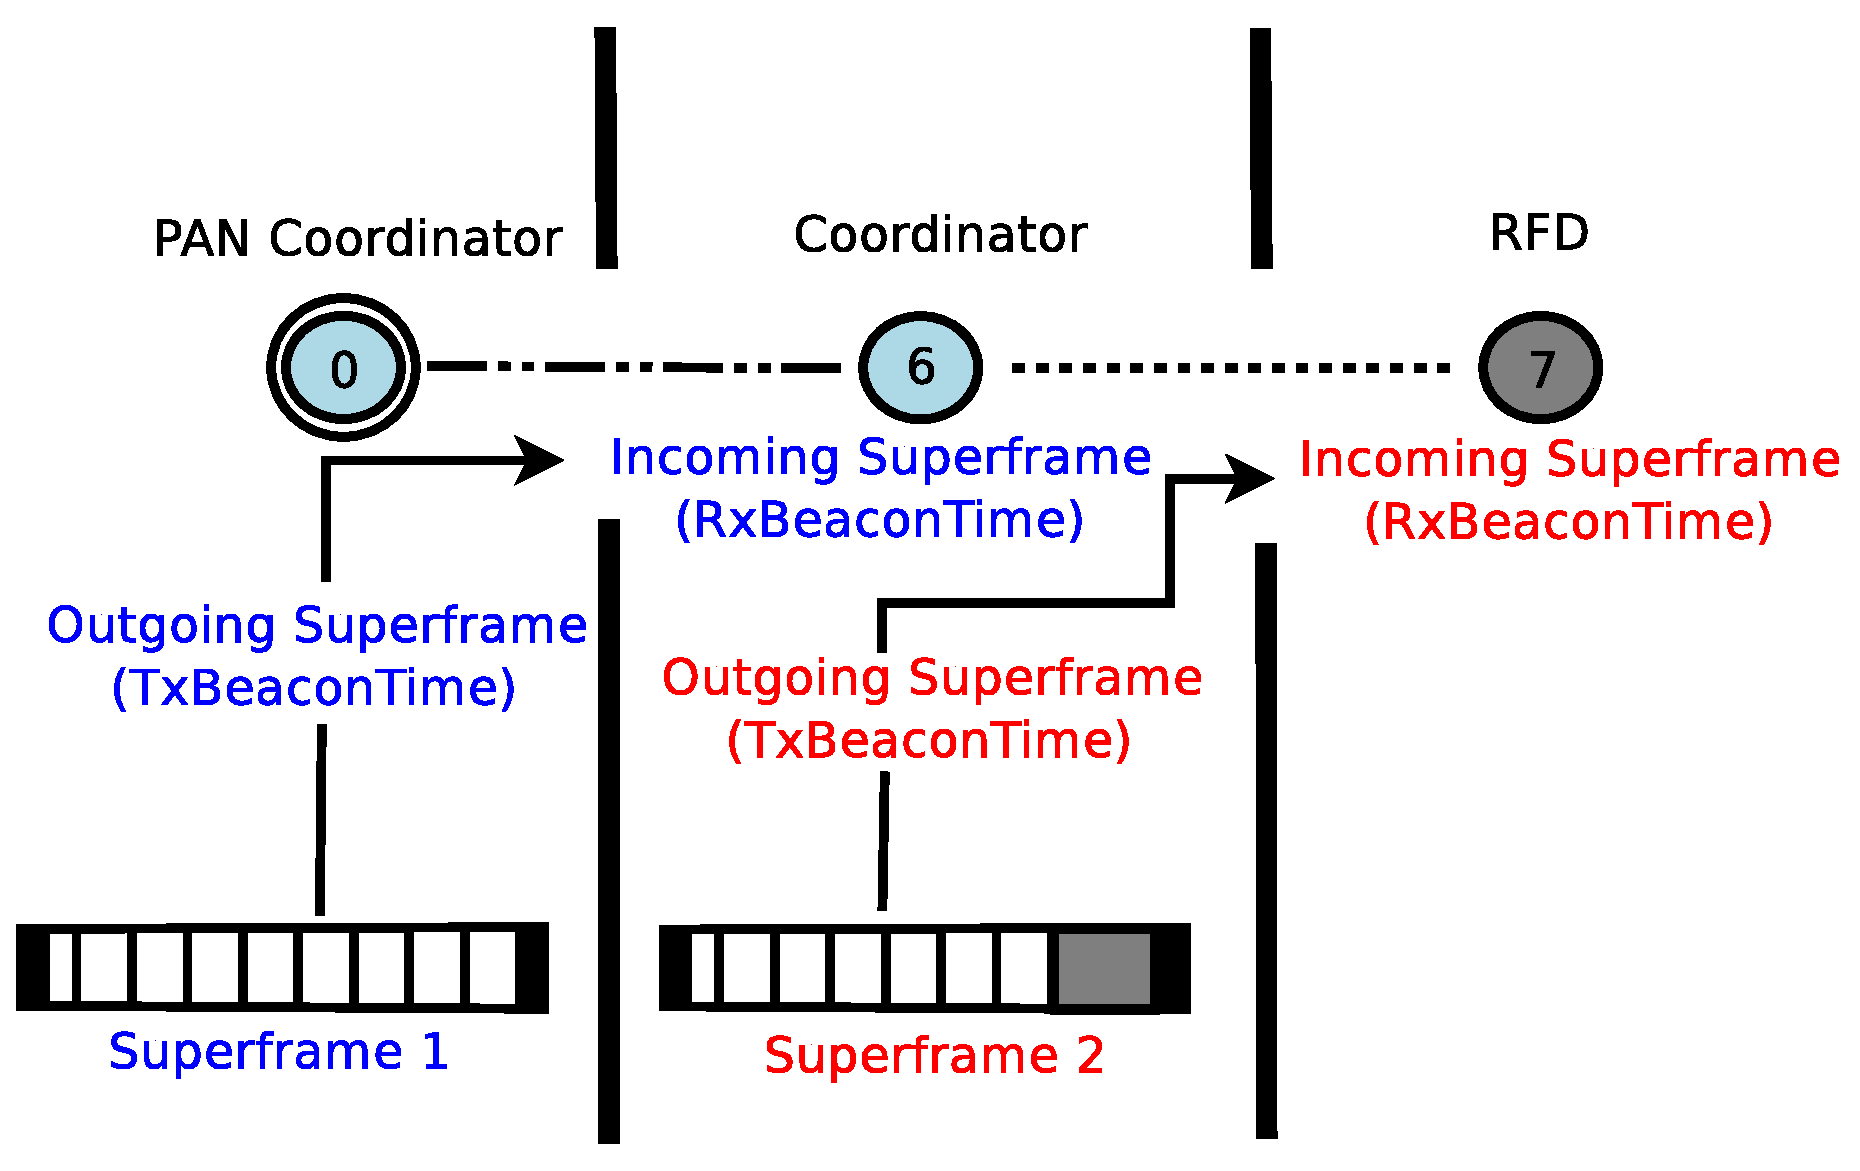
\includegraphics[scale=.28]{superframeRef}
\caption{Outgoing and Incoming superframe relationship in a Mesh Network.}
\label{fig:superframeRef}
\end{figure}

One aspect often overlooked by official \mbox{IEEE 802.15.4} standard documents and researchers is the beacon-enabled function in mesh topologies. While the standard states that this configuration is possible, little to no details are provided on the means to achieve this in multiple revisions. Figure \ref{fig:peerTopology} presents an example of the ways of achieving a mesh topology. While only one PAN coordinator exists in a star topology PAN, it is possible to have extra coordinators to create a mesh network. PAN coordinators differ from coordinators in the sense that only PAN coordinators can initialize the network (association process) and give commands to other coordinators for administering the network. Each coordinator transmits its own beacons that contain the information of its superframe. The transmitted superframe helps synchronize data transmissions between a coordinator and its associated devices. In a mesh topology, a PAN coordinator transmits a superframe to its associated devices, but also, one or more of these devices can act as coordinators and therefore, transmit another superframe to its own associated devices. The transmitted superframe is known as the outgoing superframe and the received superframe is known as incoming superframe. In Figure \ref{fig:superframeRef}, it is possible to observe this superframe relationship for one segment of the mesh network previously presented in Figure \ref{fig:peerTopology}. When the \mbox{coordinator 6} wishes to transmit data to its PAN coordinator 0, the \mbox{coordinator 6} uses the incoming superframe information \mbox{(superframe 1)}. Similarly, if the \mbox{coordinator 6} wishes to transmit data to its associated device \mbox{node 7}, it will use the outgoing superframe reference that originated from itself \mbox{(superframe 2)}. An incoming superframe uses the beacon reception time from its coordinator (RxBeaconTime) as a reference to the beginning of the superframe. An outgoing superframe uses its beacon transmission time (TxBeaconTime) as a reference to the beginning of the superframe.

\subsection{IEEE 802.15.4 (2006)}\label{wpan2006}
The 2006 revision \cite{std2006} was the first revision after the standard was introduced in 2003. In this revision, a field in the Frame Control Field (FCF) of the MAC Header was added to easily verify the version in use. The biggest changes in this revision are in the physical layer. The 2003 original 868/915 MHz bands employed a Binary Phase-Shift Keying (BPSK) modulation. Optionally, an Amplitude Shift Keying (ASK) modulation on the 868/915 MHz bands can be used in this revision. This modulation effectively increases the offered data rate to 250 kb/s for both bands. The same data rate could only be achieved on the 2450 MHz band in the 2003 revision. In addition to the 868/915 MHz bands BPSK and ASK modulations, an Optional Offset Quadrature Phase-Shift Keying (O-QPSK) modulation was added. This modulation offers an increased data rate of 100 kb/s and 250 kb/s, respectively, when compared to the original BPSK modulation. O-QPSK modulation was only possible on the 2450 MHz band in the 2003 revision. As for MAC layer enhancements, the 2006 revision enables specification beacons start times via a parameter in the MAC layer primitives. Pre-establishing the start time helps reduce beacon collisions among PAN coordinators.

\subsection{IEEE 802.15.4a (2007) - Amendment 1}\label{wpan2007}
IEEE 802.15.4a \cite{std2007} is the first amendment to the 2006 revision. It introduces two new PHYs: the Ultra-wide Band (UWB) and the Chirp Spread Spectrum (CSS). UWB operates at frequencies of 3 GHz, 5 GHz, 6 GHz to 10 GHz, and less than 1 GHz (16 channels). UWB has a maximum over-the-air data rate of 851 kb/s with optional data rates of 110 kb/s, 6.81 Mb/s, and 27.24 Mb/s using a combined modulation of Burst Position Modulation (BPM) and BPSK. On the other hand, CSS operates in the PHY 2450 MHz with supports for data rates of 1000 kb/s or 250 kb/s. The UWB enables the use of precision ranging (calculation of  the distance between two devices) using the Two-Way Ranging (TWR) protocol that enables ranging calculation without a common time reference.

\subsection{IEEE 802.15.4c (2009) - Amendment 2}\label{wpan2009c}
The second amendment\cite{std2009c} to the 2006 revision adds two extensions to the physical layer: One 780 MHz PHY with the O-QPSK modulation and another 780MHz PHY with the new modulation M-ary Phase Shift Keying (MPSK). Both these additions are meant to be used in China and have a maximum data rate of 250 kb/s, regardless of the modulation used. 

\subsection{IEEE 802.15.4d (2009) - Amendment 3}\label{wpan2009d}
Similar to 2nd, the 3rd amendment to the 2006 revision \cite{std2009d} adds extensions to the physical layer exclusively for Japan. These extensions include two additional PHY: a PHY in the 950 MHz band with a Gaussian Frequency-Shift Keying (GFSK) modulation with a maximum data rate of 100 kb/s and a PHY in the 950 MHz band using the BPSK modulation with a data rate of 20 kb/s.
\subsection{IEEE 802.15.4 (2011)}\label{wpan2011}
The 2011 revision \cite{std2011} compiles all changes made in the last 3 amendments after the 2006 revision into a single document. In this revision, the standard dropped the concept of Service Specific Convergence Sublayer (SSCS) and instead exclusively focuses on PHY and MAC layer topics. Because of the lack of a flexible MAC layer,  the 2011 revision gave birth to numerous alternative MAC layer proposals that satisfy the requirements of different types of applications. In time, the standard addressed these concerns and officially introduced variants to the MAC layers in the form of \textit{MAC behaviors} in subsequent amendments.

\subsection{IEEE 802.15.4e (2012) - Amendment 1}\label{wpan2012e}
While most amendments prior to this one focus on PHY layer additions, IEEE 802.15.4e\cite{std2012e} proposed significant changes to the MAC layer. These changes impacted the standard in 2 ways. First, it relegated the previous MAC layer to an all-purpose legacy status. Second, it reworked the MAC layer to a modular and specialized design in the form of \textit{MAC behaviors}. These MAC behaviors introduce a level of flexibility never present in the previous versions and, therefore, include a point of interest often surveyed and evaluated by researchers \cite{nutshell}. IEEE 802.15.4e describe 5 MAC behaviors: 
%Radio Frequency Identification (RFID) BLINK, Asynchronous Multichannel Adaptation (AMCA), %Deterministic Synchronous Multichannel Extension (DSME), Low Latency and Deterministic %Networks (LLDN) and Time Synchronous Channel Hopping (TSCH).

\textbf{RFID}. The standard specifies the MAC behavior called BLINK, which is a specific kind of Radio Frequency Identification (RFID) \cite{isostd}. RFID BLINK transmits encrypted data and is well suited for applications that involve sensitive information, which is the reason for its wide use in contactless credit card transactions and transportation systems worldwide. Devices connecting with RFID do not require prior association or acknowledgement. 

\textbf{AMCA}. The Asynchronous Multichannel Adaptation MAC behavior is designed to work in environments with low channel quality because of noise or the presence of a large number of devices in a non-beacon enabled network. These problems can cause link asymmetry, which leads to a rapid degradation in communication. To combat this, during an active scan, AMCA tests the link quality on all available channels through requests made by the coordinator. This way, AMCA selects the channel with the highest link quality for either listening or transmitting at any given time.

\textbf{DSME}. The Deterministic Synchronous Multichannel Extension MAC behavior is targeted at applications that require high levels of reliability or deterministic latency. Examples include applications in industrial automation in which the loss of data represents a serious problem and applications in health monitoring where a guaranteed timely response is necessary. Simultaneously, DSME can also handle densely populated networks such as sensor networks. Similar to the beacon-enabled mode in the legacy MAC, synchronized  transmissions are performed using \textit{superframes} structures, but these superframes are contained in \textit{multiframes} structures. DSME multi-superframe structures are described in Figure \ref{fig:dsmeSuperframe}. Like before, a superframe is formed by a CAP and a CFP. In DSME, a single channel is used for the association process, which involves the transmission of Enhanced Beacons (EB) and transmissions during the CAP. The EB is a new addition to the standard and is composed of Information Elements (IE). IE are introduced for the first time in this amendment but are also used in other standards such as the IEEE 802.11. IE enables a more flexible use of the fields because they possess variable sizes, greatly extending the functionality of the frame that uses them. Different from the legacy MAC beacon-enabled, the CFP in DSM is capable of allocating up to 7 GTS for each available channel (16 channels). Alternatively, the slots can be assigned to perform Group Acknowledgment (GACK). With a GACK, it is possible to combine several acknowledgments to be sent to all devices communicating within the same superframe. This feature helps reduce latency and energy consumption.
\ref{fig:dsmeSuperframe}.
\begin{figure}[!htb]
\centering
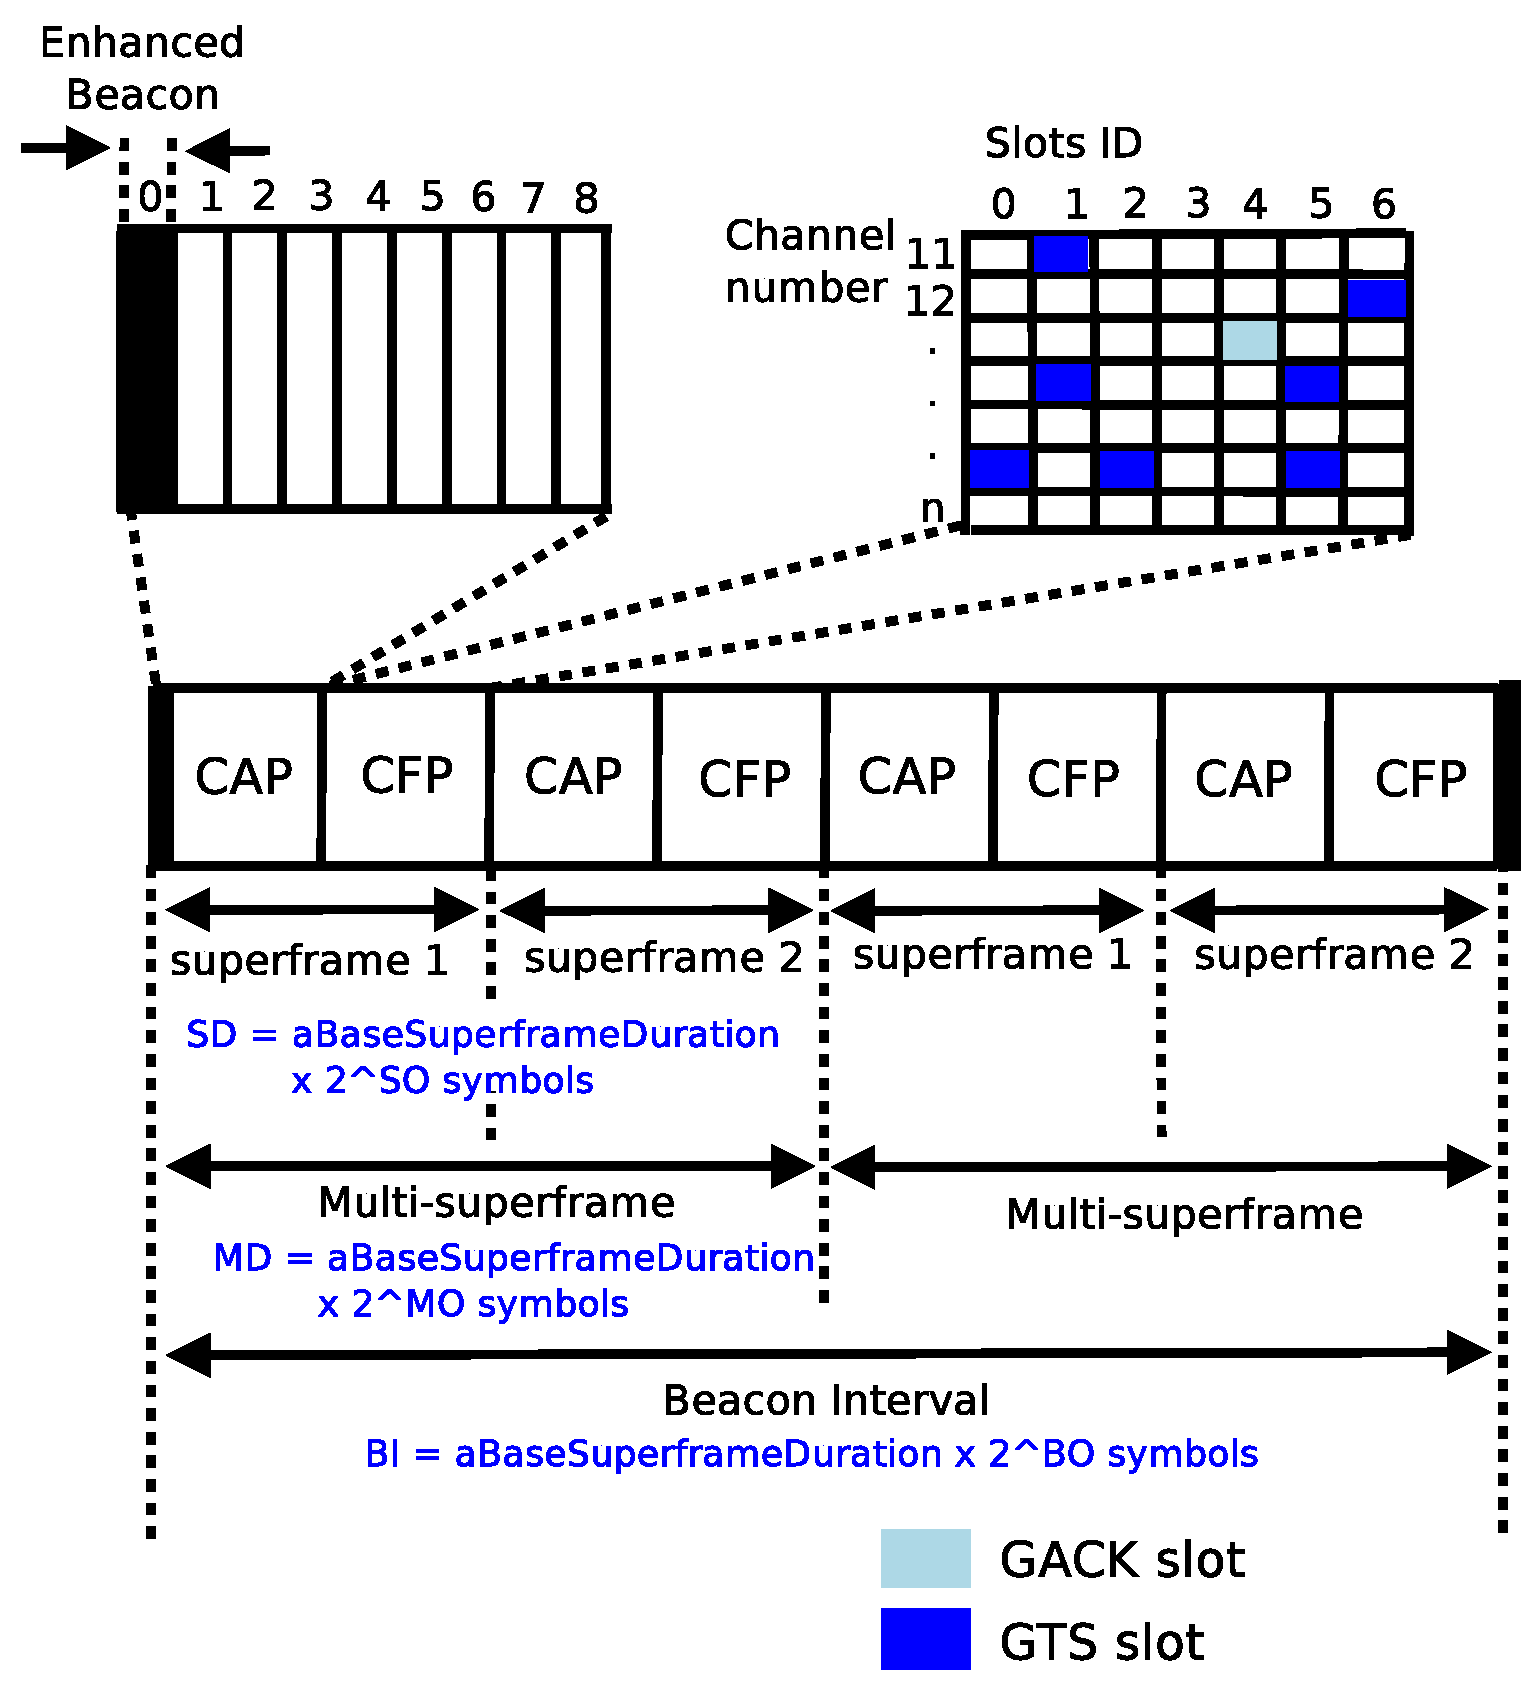
\includegraphics[scale=.28]{dsmeSuperframe}
\caption{DSME multi-superframe structure.}
\label{fig:dsmeSuperframe}
\end{figure}

 Another unique feature of DSME is CAP reduction. Except for the first superframe CAP in the multi-frame, DSME can completely eliminate subsequent CAPs in the multi-frame and use the time gained to effectively increase the time for exclusive transmissions in CFP operations. DSME Beacon Interval (BI) is equal to \mbox{$aBaseSuperframeDuration$ x $2^{BO}$} symbols where $aBaseSuperframeDuration$ is equal to 960 symbols and the Beacon Order (BO) is an integer between 0 and 14. The superframe duration (SD) is equivalent to \mbox{$aBaseSuperframeDuration$ x $2^{SO}$} symbols, where SO is the superframe order and is related to the BO in \mbox{0 $\leq$ $SO$ $\leq$ $BO$ $\leq$ 14}. Likewise, the Multi-superframe Duration (MD) is the result of \mbox{$aBaseSuperframeDuration$ x $2^{MO}$} symbols where MO is the Multi-superframe Order and relates to both SO and BO in \mbox{0 $\leq$ $SO$ $\leq$ $MO$ $\leq$ $BO$ $\leq$ 14}. To overcome interference as a result of noise present in a given channel, DSMA can check the link quality and use \textit{channel adaptation} to switch a GTS (assigned to a specific device) to a different channel in a consecutive time slot. On the other hand, \textit{channel hopping}, a well-known technique, can be used to set a predefined sequence to hop between channels during the whole frame transmission.

\textbf{LLDN}. The Low Latency Deterministic Networks MAC behavior was specifically designed for factory automation or implementations with similar requirements and limitations. LLDN is exclusive used in centralized networks (star topology) that require latencies as low as 10 ms for more than a 100 devices connected to a single coordinator. Examples of LLDN applications include, but are not limited to robots, airport logistics, conveyors, automatic packing, cargo, etc. 
\begin{figure}[!htb]
\centering
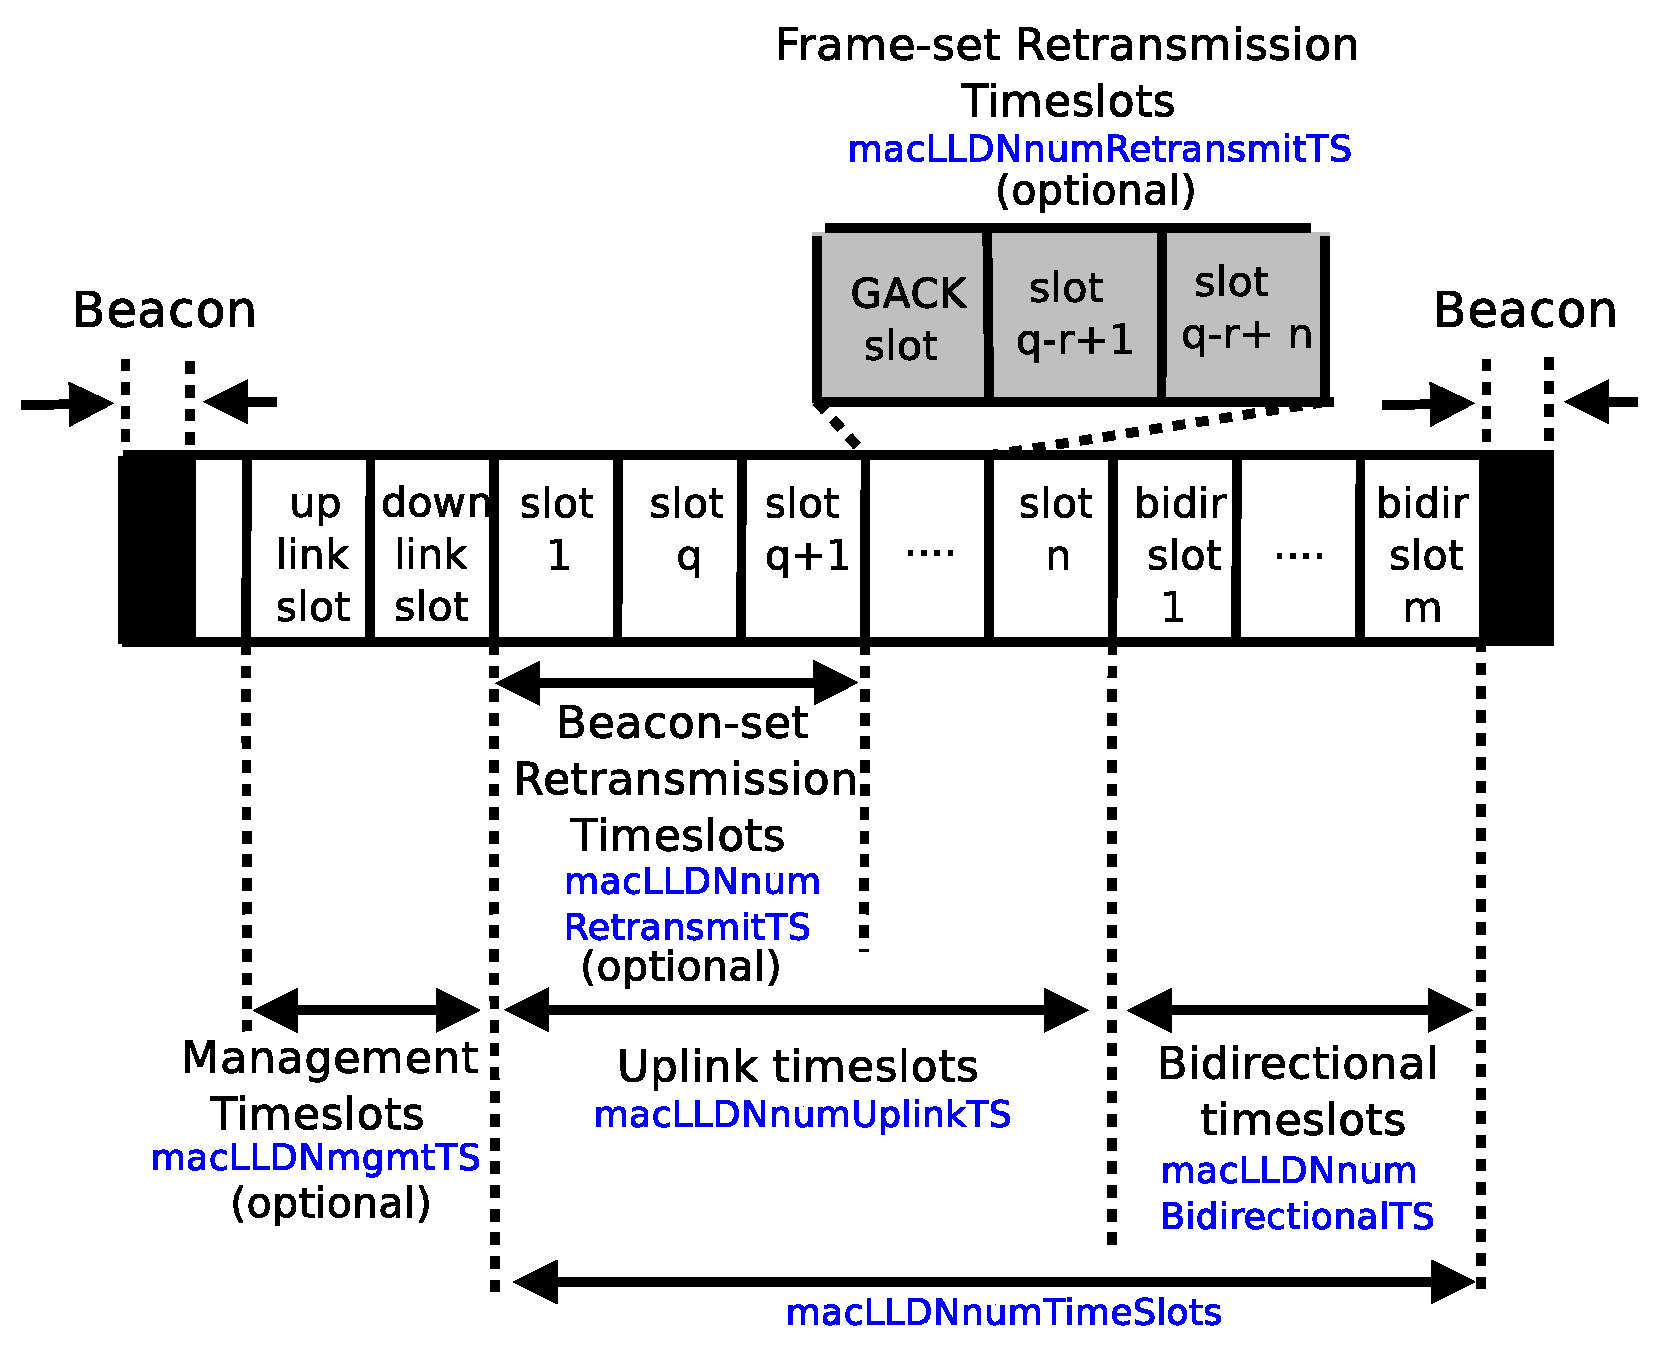
\includegraphics[scale=.28]{llframe}
\caption{LLDN superframe structure.}
\label{fig:llframe}
\end{figure}

In LLDN there can be two types of devices; devices that can only send data to the coordinator (uplink capable) or devices that can do both, send and receive data from the coordinator (uplink and downlink capable). LLDN has a \textit{superframe} structure in which the first time slot is assigned to the beacon and the remaining slots of equal size are assigned to specific devices in the network. Multiple devices can be assigned to a single slot and they contend for the medium using CSMA/CA. In LLDN, superframe time slots have a specific order and purpose: a) The \textit{beacon timeslot} which is always present. b) The \textit{management timeslots}: \textit{downlink} and \textit{uplink} timeslots. The existence of management slots is optional and depends on whether or not the \textit{macLLDNmgmtTS} flag is set true. c) The \textit{uplink timeslots} are used for transmissions from the devices to the coordinator. In addition, the first uplink slots can be used for re-transmissions if specified by the Group Acknowledgment (GACK) field in the beacon. Alternatively, re-transmissions can also be set using an LL-Acknowledgment frame (command frame) sent in the \textit{bidirectional timeslots}.  d) \textit{Bidirectional timeslots} are used for multi-link communication between the coordinator and its devices. The slot size and number of slots for each usage are indicated by the \textit{macLLDN} attributes, as shown in Figure \ref{fig:llframe}.

\textbf{TSCH}. The Time Slotted Channel Hopping MAC behavior was created for robustness. TSCH applications include the oil and gas industry, chemical and pharmaceutical production, or applications prone to collisions caused by the saturation of the network. TSCH considers a deterministic response as the most important aspect of communication. Different to DSME, TSCH support mesh and star topologies. In TSCH, \textit{superframes} are replaced with \textit{slotframes}. Slotframes repeat cyclically and are formed by a sequence of \textit{timeslots}. Each timeslot has an incremental Absolute Slot Number (ASN) that indicates the total number timeslots elapsed since the beginning of the network. Transmissions inside these timeslots can occur with or without contention. In addition, in TSCH, it is possible to use concurrent slotframes, each with independent timeslot configurations. However, all slotframes are aligned to the same timeslot boundaries. Unlike the channel diversity used in DSME, TSCH relies on a channel hopping mechanism to achieve communication. The frequency $f$ used in a transmission between two nodes is defined by \mbox{$f= F[(ASN+ channel Offset) \% NChannels]$} where \textit{channel Offset} is an integer between 0 and 15, \textit{NChannels} is the hopping sequence length, and $F$ denotes a lookup table. In this manner, a different frequency is obtained for the same link in different time slots. TSCH behavior is summarized in Figure \ref{fig:tschSlotframe}.
\begin{figure}[!htb]
\centering
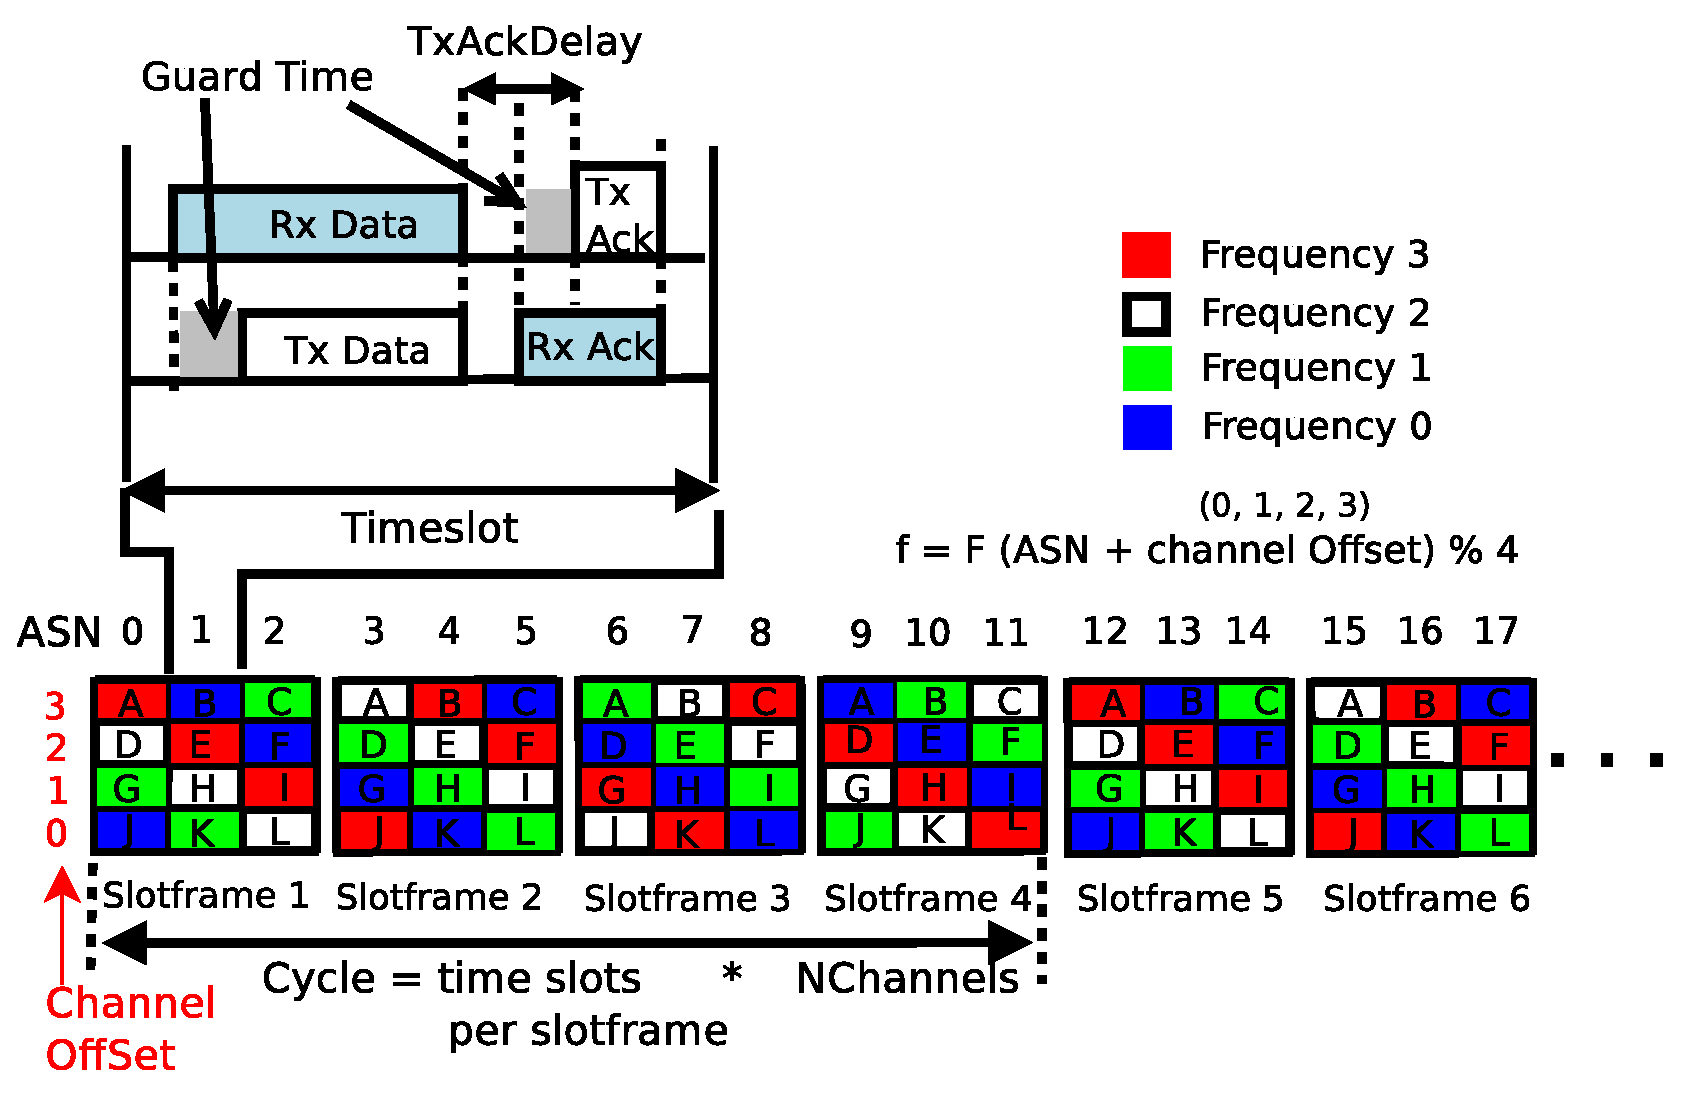
\includegraphics[scale=.28]{tschSlotframe}
\caption{TSCH frequency hopping mechanism.}
\label{fig:tschSlotframe}
\end{figure}
\subsection{IEEE 802.15.4f (2012) - Amendment 2 }\label{wpan2012f}
 The 2nd amendment \cite{std2012f} to the 2011 revision has two new PHY. First, the Low-rate PRF Ultra-Wide Band (LRP UWB) optimized for low complexity RFID transmitters (tags) exhibits a level of interoperability  only present with the UWB PHY in previous revisions. LRP UWB offers 3 modes: a) \textit{Base mode} with an OOK modulation and a bit rate of 1000 kb/s. b) \textit{Extended mode} with an OOK modulation and a bit rate of 250 kb/s. c) \textit{Long-range mode} with a Manchester PPM modulation and a maximum bit rate of 31.25 kb/s. The second PHY is a 2450 MHz band PHY with a Minimum Shift Keying (MSK) modulation and a maximum bit rate of 250 kb/s for RFID applications. The 2450 MHz band is the Industrial, Scientific and Medical (ISM) band and therefore devices operate on this band (e.g. Wi-fi, ZigBee). Moreover, small unused gaps in the spectrum on the edges of these frequencies tend to exist. MSK 2450MHz PHY takes advantage of those spaces and is capable of using up to 42 possible narrowband channels that fall on these unused gaps, gracefully coexisting with existing devices using the same band. Alternatively, MSK can operate on the much less saturated 433 MHz band with bit rates of 31.25, 100 or 250 kb/s.
\subsection{IEEE 802.15.4g (2012) - Amendment 3 }\label{wpan2012g}
IEEE 802.15.4g \cite{std2012g}, known as the Smart Utility Networks (SUN) standard, was created to be used in the emerging Smart Grids (SG). SGs are electrical grids capable of bidirectional energy flow and communication \cite{smartGrid}. SUN PHYs are often used in smart metering applications with long-range, low-power requirements. This amendment introduces three PHY with multiple data rates to choose from. The PHY names are described by its modulation names: a) Multi-Rate and multi-regional Frequency Shift Keying (MR-FSK). b) Multi-Rate and multi-regional Offset Quadrature Phase-Shift Keying (MR-O-QPSK), which shares characteristics with the 2011 modulation O-QPSK. c) The Multi-Rate and multi-regional Orthogonal Frequency Division Multiplexing (MR-OFDM), which uses DSSS and MDSSS. Some of the SUN PHY frequencies established in this amendment have been revised in later amendments.
\subsection{IEEE 802.15.4j (2013) - Amendment 4 }\label{wpan2014j}
This amendment \cite{std2013j} introduces a single PHY for the 2380 MHz band with a maximum bit-rate of 250 kb/s. Its use is restricted to transmission data (no voice) in devices for monitoring, diagnosing, and treating of patients. These devices must be compliant with the Federal Communications Commission (FCC) rules for Medical Body Area Networks (MBAN).
\subsection{IEEE 802.15.4k (2013) - Amendment 5 }\label{wpan2014k}
This amendment added 2 more PHYs: a) A DSSS PHY with either BPSK or O-QPSK modulation schemes. b) A FSK PHY with 3 possible modulations; a Gaussian FSK (GFSK), Position-based FSK (P-FSK), and Position-based Gaussian FSK (P-GFSK). These PHY are designed for Low Energy, Critical Infrastructure Monitoring (LECIM) applications. LECIM operates on a wide range of frequencies \cite[pp. 58-61]{std2013k} with multiple data rate options for each of these modulations. One of its main features is the ability to use the priority channel access (PCA). PCA enables the allocation of high-priority messages in the CAP period of the superframe structure. Experiments performed by Gebremedhin et al.\cite{experimentK} demonstrated that under some conditions, PCA messages can greatly improve the latency of emergency messages while slightly affecting the performance of normal messages.
\subsection{IEEE 802.15.4m (2014) - Amendment 6 }\label{wpan2014m}
The amendment objective was to re-purpose the unused frequency space left between TV channels in UHF bands. Originally, this space was left unused to prevent TV channels from interfering with one another. This space is known as TV White Space (TVWS) and its value depends on its potential for longer range communications. A 2.4 Ghz signal might travel several kilometers in the right conditions, however, UHF (470 - 698 MHz) can travel for many miles. However, it is worth noting that existing TVWS (i.e. 600 - 700 MHz) are increasingly becoming unavailable because of an increasing demand in cellular frequencies. TVWS PHY support multiple data rates in bands ranging from 54 MHz to 862 MHz, aided by 3 modulation schemes: TVWS-FSK, TVWS-OFDM, and TVWS-NB-OFDM. The coexistence of IEEE 802.15.4m with other standards using TVWS have been explored in \cite{coexistence}.
\subsection{IEEE 802.15.4p (2014) - Amendment 7 }\label{wpan2014p}
This amendment \cite{std2014p} addressed the need for a communication standard in Rail Communications Control (RCC) systems. This standard enabled data rates of up to 1 Mbit/s over frequencies in the VHF, UHF, and SHF bands (161, 216, 217, 220, 450, 770, 896, 915, 928, 2450, 4965, 5800 MHz) operating in contiguous and non-contiguous channel bandwidths as narrow as 12.5 kHz and as wide as 2Mhz. The standard includes multiple modulation technique options: GMSK, QPSK, and DPSK among others. A full list of the frequencies and modulations introduced for this amendment can be found in \cite[pp. 386]{std2015}.
\subsection{IEEE 802.15.4 (2015) }\label{wpan2015}
IEEE 802.15.4-2015 \cite{std2015} is the third revision of the standard. As its predecessors, this combines all the PHYs additions and MAC enhancements since the 2011 revision in a single document. Additional corrections to the document are editorial in nature. 
\subsection{IEEE 802.15.4n (2016) - Amendment 1 }\label{wpan2016n}
The first amendment \cite{std2016n} to the 2016 revision present another PHY alternative for the transmission of medical information in China. The China Medical Band (CMB) defines the 174-216 MHz, 407-425 MHz, and 608-630 MHz bands for this purpose and restricts its use for voice applications.
\subsection{IEEE 802.15.4q (2016) - Amendment 2 }\label{wpan2016q}
IEEE 802.15.4q \cite{std2016q} introduced two PHY for 2.4 GHz and multiple sub-gigahertz bands with data rates up to 1 Mb/s. These PHYs were designed for ultra low-cost (low complexity) and ultra-low power applications. To achieve this, the standard used two new modulations: the Rate Switch Gaussian Frequency Shift Keying (RS-GFSK) and the Ternary Amplitude Shift Keying (TASK). RS-GFSK provided options for working alongside existing SUN FSK PHYs. Consequently, smart metering, smart irrigation, and home network applications benefit from these PHYs.
\subsection{IEEE 802.15.4u (2016) - Amendment 3 }\label{wpan2016u}
The third amendment to the 2015 revision \cite{std2016u} brought the 866 Mhz PHY to India. This PHY defined the 865-867 MHz band with an option for multiple bit-rates to choose from and 3 possible modulations: SUN FSK, OFDM, O-QPSK.
\subsection{IEEE 802.15.4t (2017) - Amendment 4 }\label{wpan2017t}
A new PHY was introduced in this amendment \cite{std2017t}, which was designed to operate on devices that require a short burst of information at high speeds (up to 2 Mb/s) followed by long sleep periods, contributing to extended battery life. This amendment uses the same 2400-483.5 MHz frequencies occupied by the O-QPSK PHY in place of MSK modulation.
\subsection{IEEE 802.15.4v (2017) - Amendment 5 }\label{wpan2017v}
This amendment \cite{std2017v} changed multiple SUN PHY frequency ranges, including their channel ranges. The changes conceded the use of the 870-876 MHz and the 915-921 Mhz in Europe, the 902-928 MHz in Mexico, the 902-907.5 in Brazil and the 915-928 MHz in Australia, Brazil, and New Zealand. In addition, frequency range changes are made to the LECIM and TVWS PHYs.
\subsection{IEEE 802.15.4s (2018) - Amendment 6 }\label{wpan2018s}
IEEE 802.15.4s \cite{std2018s} is the latest amendment to date. In this amendment, several MAC layer primitives and commands were added as part of the Spectrum Resource Measurements (SRM) toolkit. These changes are the most significant additions to the MAC layer since 802.15.4e-2012. SRM enables the  measure, transmission, and request of information concerning the state of the channel. The MAC layer can report this information to higher layers for its usage. Some of the SRM introduced features include:





\begin{itemize}
  \setlength{\itemsep}{1pt}
  \setlength{\parskip}{0pt}
  \setlength{\parsep}{0pt}
  \item \textit{Failed Transmissions measurement.} It estimates the propagation quality of specific links as part of the channel selection algorithm.
  \item \textit{Deferred Transmissions measurement.} It helps to determine the level of congestion in the channel caused by other coexisting networks.
  \item \textit{Retry Histogram.} It provides a histogram with the number of retries from a single transmission during a determinate space of time.
  \item \textit{Noise Histogram.} Reports the noise power of non-IEEE 802.15 devices in a specific channel during a specific period of time.  
  \item \textit{Channel Usage.} Display the total Channel time used during a sequence of Rx and Tx frames during a period of time.
  \item \textit{Received Signal Strength Indicator (RSSI)}
  \item \textit{Energy Detection (ED).}
\end{itemize}

Table \ref{tab:phyTable} summarizes all the standard PHY except for the extensive RCC, LECIM, SUN and TVWS PHYs which constantly changed.


 %[\begin{table}!htbp]
\begin{table}[!htbp]
%\begin{center}
\caption{IEEE 802.15.4 PHY evolution.}
\label{tab:phyTable}
{\renewcommand{\arraystretch}{1.2}
\begin{tabular}{|c|@{}c@{}|@{}c@{}|@{}c@{}|@{}c@{}|@{}c@{}|}
\hline
 \begin{tabular}{@{}c@{}}\textbf{PHY}\\ \textbf{(MHz)}\end{tabular} & 
 \begin{tabular}{@{}c@{}}\textbf{Band} \\ \textbf{(MHz)}\end{tabular} & 
 \begin{tabular}{@{}c@{}}\textbf{\scalebox{0.8}{Modulation -}} \\ \textbf{\scalebox{0.8}{Spread Spectrum}}\end{tabular} &  
 \begin{tabular}{@{}c@{}}\textbf{Bit-Rate}\\\textbf{(kb/s)}\end{tabular} & 
 
 \begin{tabular}{@{}c@{}}\textbf{Symbol}\\\textbf{Rate} \\ \textbf{(ksym/s)}\end{tabular} \\ \hline
 
 
 \begin{tabular}[c]{@{}c@{}}2450 \scalebox{0.8}{(World Wide)} \\ \scalebox{0.8}{IEEE 802.15.4-2003}\end{tabular} &  \begin{tabular}{@{}c@{}} 2400 - \\ 2483.5\end{tabular} & O-QPSK \scalebox{0.8}{*DSSS} & 250 & 62.5 \\ \hline





915 \scalebox{0.8}{(U.S.A)}  & 902 - & BPSK & 40 & 40 \\ \cline{3-5}
\scalebox{0.8}{IEEE 802.15.4-2003} & 928 & ASK \scalebox{0.8}{*PSS}& 250 & 50 \\ \cline{3-5}
     &   & O-QPSK & 250 & 62.5 \\ \hline





868 \scalebox{0.8}{(Europe)}  & 868 - & BPSK & 20 & 20 \\ \cline{3-5}
\scalebox{0.8}{IEEE 802.15.4-2003} & 868.6 & ASK \scalebox{0.8}{*PSS}& 250 & 12.5 \\ \cline{3-5}
     &   & O-QPSK & 100 & 25 \\ \hline

              
 
2450   & 2400-2483.5 & DQPSK$\,\to\,$  & 250 / &  166.667 / \\
\scalebox{0.8}{IEEE 802.15.4a-2007} &    & DQCSK \scalebox{0.8}{*CSS} & 1000         &                166.667 \\
\hline 

   
   
  
   
UWB sub-Ghz  & 250-750    &          & 110/850& \scalebox{0.8}{0.12/0.98(Mhz)}  \\
\cline{4-5}
sub-Ghz/low/high & 3244-4742  & BPM-BPSK & 6810 & 7.80(Mhz)  \\
\cline{4-5}
\scalebox{0.8}{IEEE 802.15.4a-2007} & 5944-10234 &          & 27240& 15.60(Mhz)  \\
\hline   
   
   
   
 780 \scalebox{0.8}{(China)}\    
 & 779 - & O-QPSK & 250 & 62.5 \\ \cline{3-5}
\scalebox{0.8}{IEEE 802.15.4c-2009} 
&787 & MPSK & 250 & 62.5 \\ \hline

    

 950 \scalebox{0.8}{(Japan)}\    
 & 950 -& GFSK & 100 & 100 \\ \cline{3-5}
\scalebox{0.8}{IEEE 802.15.4d-2009} 
&956  & BPSK \scalebox{0.8}{*DSSS}  & 20 & 20 \\ \hline



433 / 2450 & 433.05-434.79 & MSK & \scalebox{0.8}{31.25/100/250}& \scalebox{0.8}{31.25/100/250}  \\ 
\cline{2-2}\arrayrulecolor{white}\cline{3-3}\arrayrulecolor{black}\cline{4-5}
\scalebox{0.8}{IEEE 802.15.4f-2012} & 2400-2483    &     & 250 &250 \\
% \multicolumn{1}{r|}{250} & \multicolumn{1}{r|}{250}  \\
\hline   
   
   
   
  
 LRP UWB & 6289.6- & PPM & 31.25                         & 31.25            \\ 
\cline{3-5}
\scalebox{0.8}{IEEE 802.15.4f-2012} & 9185.6  & OOK & 250/1000 & 250/1000\\
\hline 
  
  
  
\begin{tabular}{@{}c@{}} 2380 \\ \scalebox{0.8}{IEEE 802.15.4j-2013}\end{tabular}   & 
\begin{tabular}{@{}c@{}} 2360 - \\ 2400\end{tabular}  
&O-QPSK \scalebox{0.8}{*DSSS}& 250 & 62.5 \\ \hline  
 

 



 195 / 416 / 619& 174-216 & \multirow{2}{*}{GFSK} & \multirow{2}{*}{50/100/200} & \multirow{2}{*}{50/100/200}  \\
\scalebox{0.8}{(China)} & 407-425 &   &   &      \\ 
\arrayrulecolor{white}\cline{2-2}\arrayrulecolor{black}\cline{3-5}
 \scalebox{0.8}{IEEE 802.15.4n-2016} & 608-630 & O-QPSK & 250/500    & 62.5/125 \\
\hline


%\scalebox{0.5}{(BPSK,QPSK,16QAM)} 
 %8.33/8.33/8.33    
   
   
                          &         & MR-FSK(2FSK)& 50/100/150              & 50/100/150  \\ 
\cline{3-5}
866 \scalebox{0.8}{(India)} &         & MR-OFDM   & 50/100/150              &   \scalebox{0.8}{8.33/8.33/8.33 }       \\
\scalebox{0.8}{IEEE 802.15.4u-2016}& 865-867 & \scalebox{0.7}{(BPSK,QPSK,16QAM)} & 200/300   &   \scalebox{0.8}{8.33/8.33}        \\ 
\cline{3-5}
                          &         & MR-O-QPSK & 6.25/12.5/25            &   100/200          \\
                          &         & \scalebox{0.8}{*DSSS}          & 50 &             \\
\hline   
   
      
\begin{tabular}{@{}c@{}} 2450 \\ \scalebox{0.8}{IEEE 802.15.4t-2017}\end{tabular}   
& 
\begin{tabular}{@{}c@{}}2400-\\2483.5\end{tabular}   
  & MSK & 2000 & 250  \\ \hline 
    
    
       
\end{tabular}
}
%\end{center}
\end{table}



\section{IEEE 802.15.4 implementations} \label{implementationStd}
At times, the accuracy of simulation results can be questionable; however, without the simulation results, large scale and costly experiments cannot be performed. The IEEE 802.15.4 is a popular protocol with multiple revisions. Despite its popularity, new revisions are gradually being adopted. By far, the 2003 and 2006 revisions are the most implemented. 2012 revisions or later, brought highly specialized PHYs and MAC behaviors limited to specific industries and applications. Their implementation in simulations is somehow rare in comparison to the legacy standard. Examples of popular IEEE 802.15.4 implementations include the following: 

The Ns-2 WPAN  module \cite{ns2implementation} is among the first simulations of the standard. Its latest version (2.35)  completely supports the IEEE 802.15.4-2003 protocol, and is to date, one of the most complete implementations of the standard with beacon and non-beacon support for mesh and star topologies (No support for inactive periods). Unfortunately, it exhibits certain disadvantages that were inherited from ns-2; lack of documentation and coding standards, unrealistic packet formats, unnecessary overhead, and lack of maintenance. Its modules are coded in C++ while scenarios require OTcl scripting language.

 Castalia (v3.3) \cite{castalia} is an OMNET++ based simulator. In addition to the basic 802.15.4-2006 MAC standard, Castalia supports 3 more MAC layers: TunableMac, TMAC, and IEEE 802.15.6. Castalia only supports beacon-enabled modes in star topologies with the optional GTS (No support for non-beacon, Indirect-transfers or mesh topology). Castalia supports PHYs modulations QPSK, BPSK, PSK, and FSK, unlike the 2006 revision of the standard. C++ and NED languages are used in OMNET++ modules. 
 
  Ns-3 \cite{ns3} is a simulator with an active community that develops new modules. Some of these modules even include emulation and hardware integration support. The latest version of the Ns-3 (V3.29) LR-WPAN module supports a full PHY  IEEE 802-15.4-2006 set with a non-beacon mode MAC for a star topology PAN (No association or beacon-enabled mode MAC options). The module exhibits promising performance; however, the module still has several limitations compared to other simulators. Its code base is C++ and it supports Python bindings.

The OPNET simulator provides an IEEE 802.15.4-2003 model \cite{opnet} that supports beacon-enabled modes in star typologies (No support for association, Non beacon-enabled mode or mesh topology). Similar to OMNET++, OPNET provides a robust GUI. Modules are build using Proto-C, C, or C++. A major drawback of OPNET is the requirement of a license.

OpenZB \cite{openzb} is an open source, real hardware implementation of the IEEE 802.15.4-2003 with beacon-enabled modes for star and mesh topologies on CrossBow MICAz and TelosB motes. OpenZB is completely programmed using the nesC language (TinyOS).


\section{Conclusions} \label{conclusions}
In this paper, we presented a historical compendium of the IEEE 802.15.4, a popular wireless standard. The standard has evolved from its humble beginnings and has been extended to handle monitoring, medical, and train network communications applications, and in recent times, grid network applications. In addition to annual revisions, our research demonstrates that simulations and hardware implementations of the standard are rarely complete and even popular simulators do not include the most recent and specialized revisions of the standard. Future IoT network performance will depend on the choice of standard selected by network specialists for a particular application and the ability of these standards to support smooth coexistence with other networks. With, literally, thousands of possible combinations to choose from, these specialists will have to depend more on simulations and a careful selection of the network features.  
 

 

 

\bibliographystyle{IEEEtran}
\bibliography{evolution802_15}


%\begin{IEEEbiography}[{\includegraphics[width=1in,height=1.25in,clip,keepaspectratio]{mshell}}]{Alberto Gallegos}
% or if you just want to reserve a space for a photo:

\begin{IEEEbiography}[{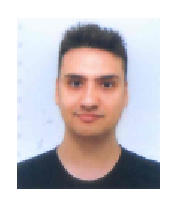
\includegraphics[width=1in,height=1.25in,clip,keepaspectratio]{Gallegos.eps}}]{Alberto Gallegos}
Received his M.S. and PH.D. degrees in Engineering from Ritsumeikan University in 2014 and 2018 respectively. He joined the College of Information Science and Engineering at Ritsumeikan University in 2018, where he is currently Assistant Professor. His current research interests include but are not limited to Wireless Sensor Networks, data mining, routing protocols, MAC layer designs and Internet of things applications.
\end{IEEEbiography}
\vspace{-17cm}
\begin{IEEEbiography}[{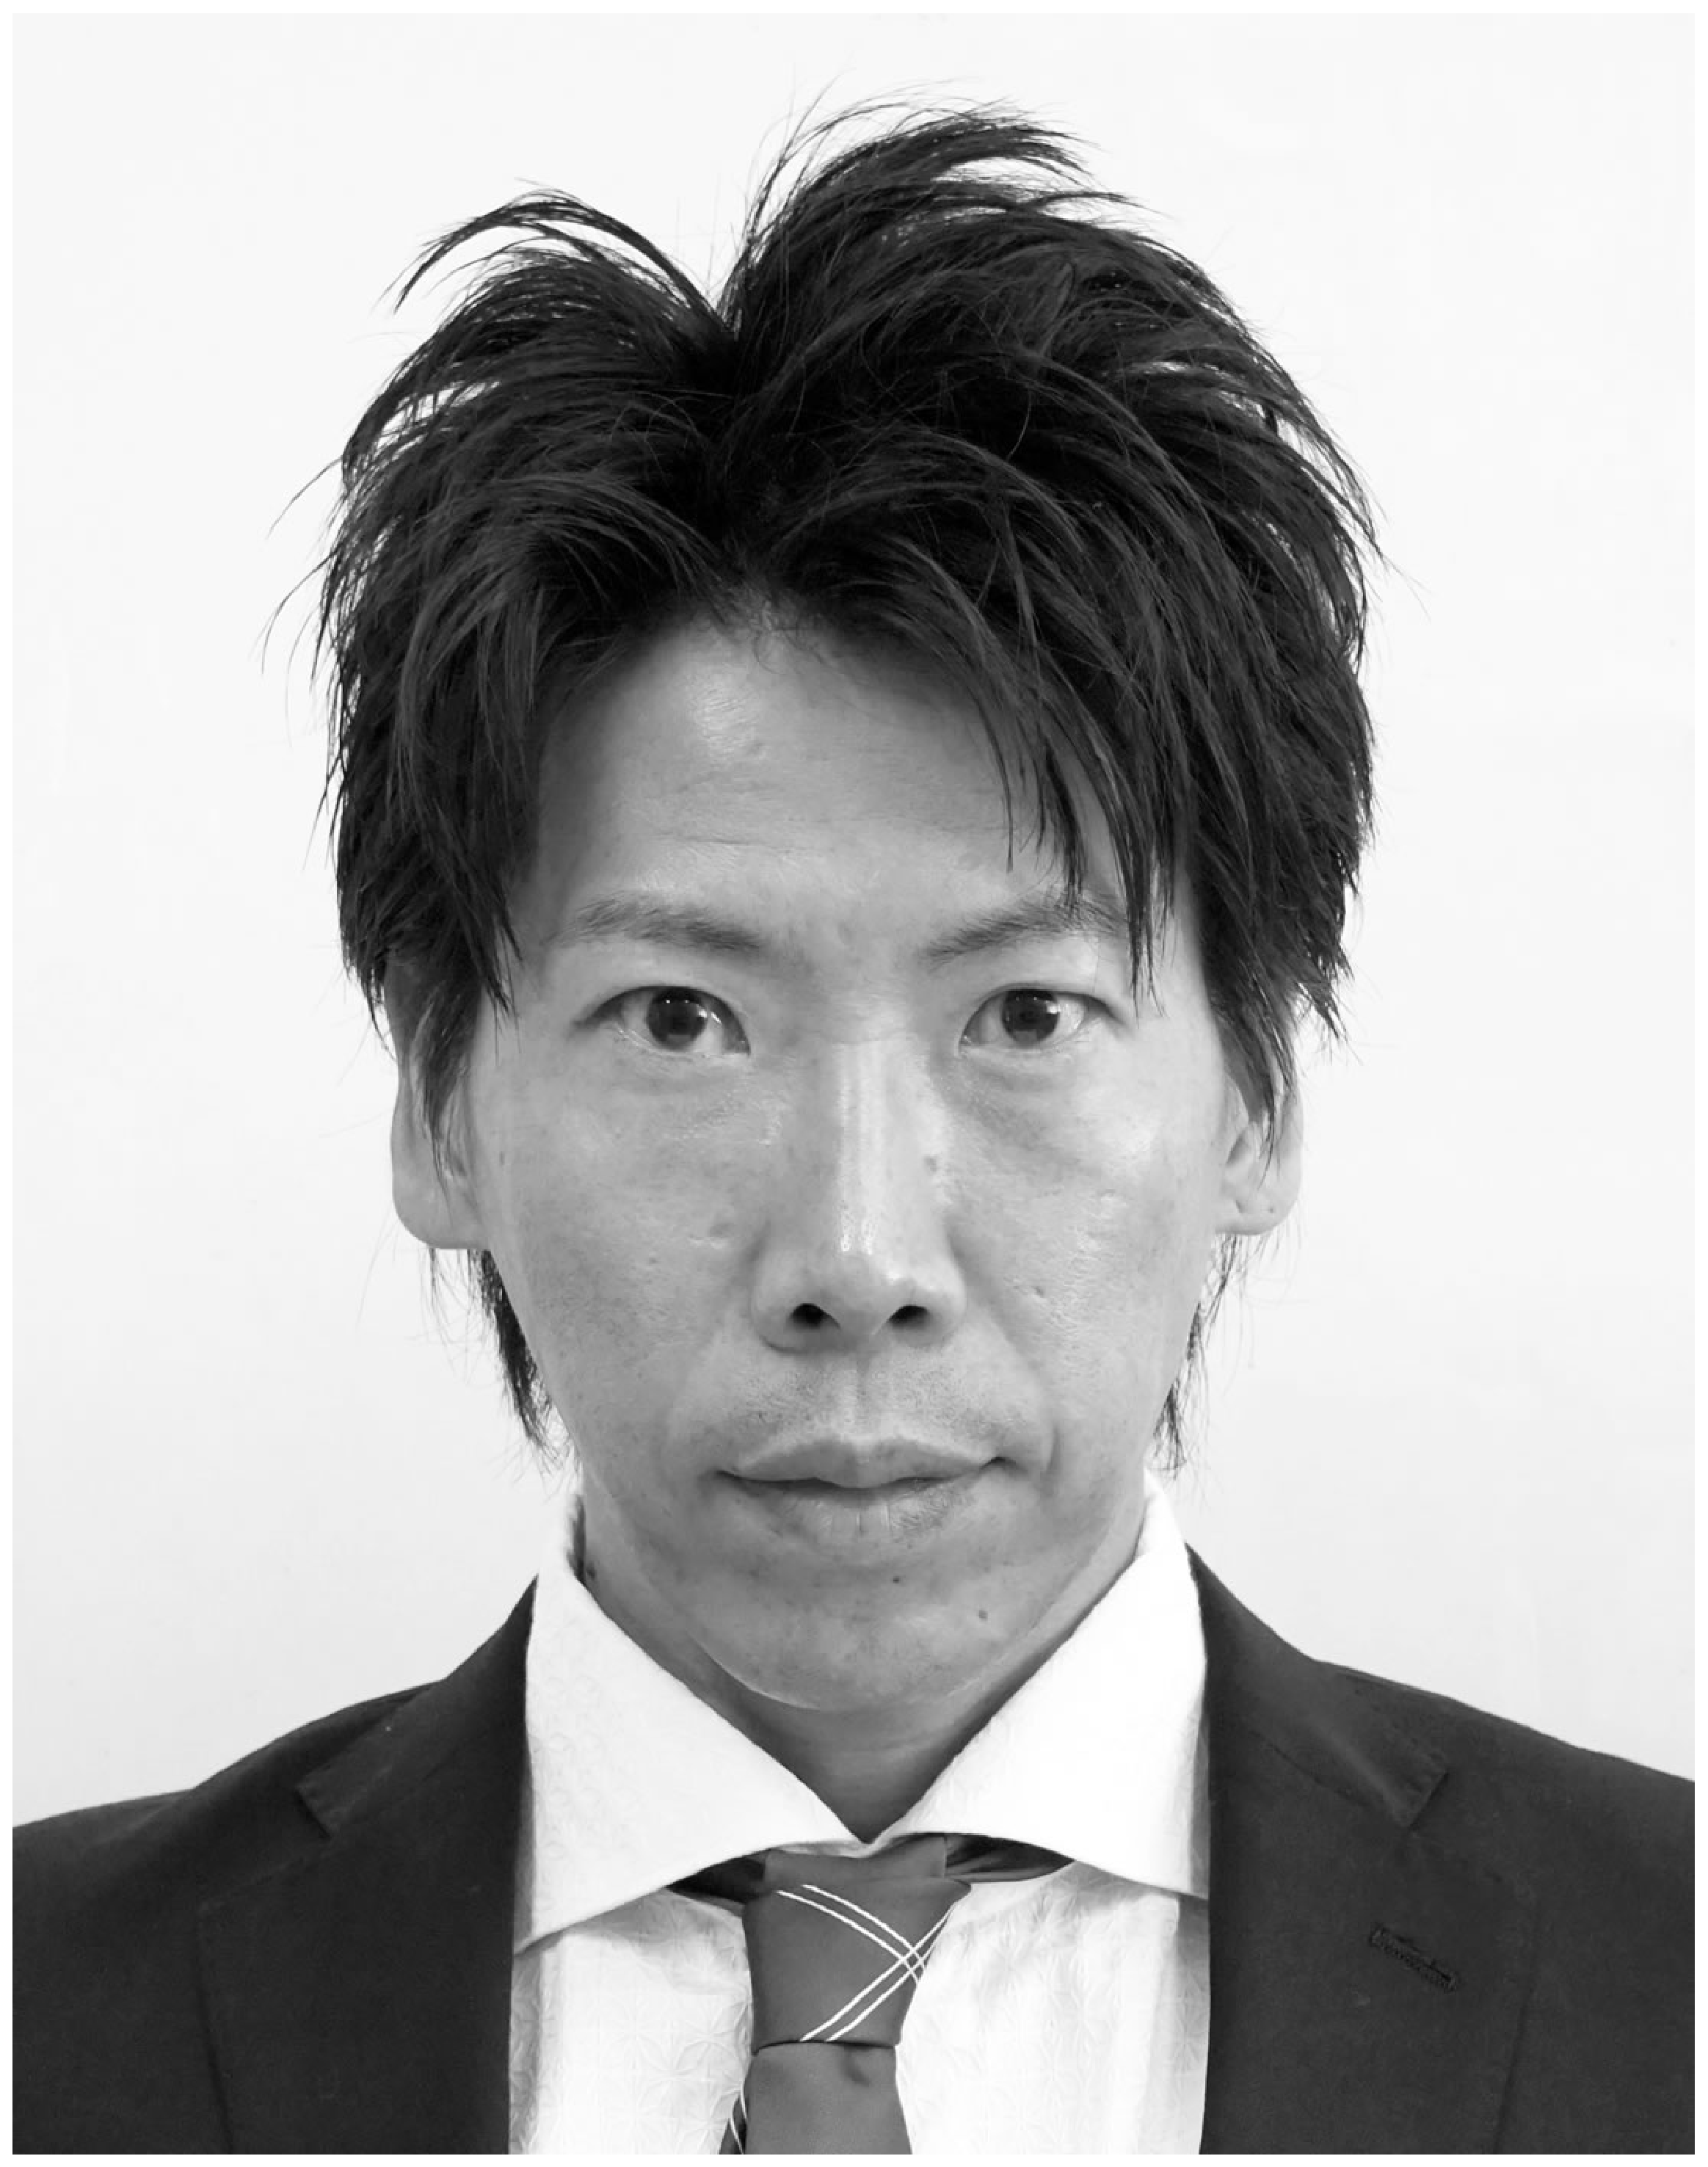
\includegraphics[width=1in,height=1.25in,clip,keepaspectratio]{NoguchiTaku.eps}}]{Taku Noguchi}
Received his B.E., M.E. and Ph.D. degrees in communications engineering from Osaka University in 2000, 2002 and 2004, respectively. He joined College of Information Science and Engineering at Ritsumeikan University in 2004, where he is currently a Professor. His research interests include performance analysis and the design of computer networks and wireless networks. He is a member of IEEE, IEICE and IPSJ.
\end{IEEEbiography}




\end{document}



